

%\documentclass[aps,twocolumn,secnumarabic,balancelastpage,amsmath,amssymb,nofootinbib, floatfix]{revtex4}
\documentclass[aps,twocolumn,secnumarabic,balancelastpage,amsmath,amssymb,nofootinbib,floatfix]{revtex4-1}

\usepackage{graphicx}
\usepackage{physics}
\usepackage{tabularx}
\usepackage{booktabs}
\usepackage{bm}
\usepackage{float}
\usepackage[colorlinks=true]{hyperref}


\begin{document}
\title{Measuring Shockley-Read-Hall Temperature Dependence of Dark Current in a CosmicWatch Silicon Photomultiplier}
\author{Ethan Suresh}
\email{easuresh@mit.edu}
\author{Max Misterka}
\email{misterka@mit.edu}

\date{\today}
\affiliation{MIT Department of Physics}


\begin{abstract}
Silicon photomultipliers (SiPMs) operated in Geiger mode generate a temperature-dependent dark count rate arising from thermally generated electron-hole pairs in the depletion region. We measure the count rate $R(T)$ of a CosmicWatch 
desktop muon detector across $T = 8$--$55\,^{\circ}\text{C}$, observing a sharp rise in the total count rate at $T = 55\,^{\circ}\text{C}$ that cannot be explained by apparatus-dependent effects. 
Applying a Shockley-Read-Hall (SRH) Arrhenius model, we identify two distinct temperature regimes separated near $T_c = 50\,^{\circ}\text{C}$, 
with extracted activation energies $E_a^{\mathrm{low}} = -0.024 \pm 0.01\,\text{(stat.)} \pm 0.03\,\text{(sys.)}\,\text{eV}$ for $T < T_c$ and $E_a^{\mathrm{high}} = 2.4 \pm 0.8\,\text{(stat.)} \pm 0.8\,\text{(sys.)}\,\text{eV}$ for $T \geq T_c$. The high-$T$ result is consistent 
with Pagano et.al's result within 1.2$\sigma$, while the low-$T$ result deviates from the Pagano et.al's value by approximately $20\sigma$, possibly due to high background radiation or impurity concentrations. Our results confirm the temperature stability of the 
CosmicWatch detector against dark current effects from $T = 8$ to $50\,^{\circ}\text{C}$.
\end{abstract}

\maketitle


%%%%%%%%%%%%%%%%%%%%%%%%%%%%%%%%%%%%%%%%%%%%%%%%%%%%%%%%%%%%%%%%%%
\section{Introduction}

The Earth's atmosphere is filled with a continuous flux of ionizing radiation including gamma rays, alpha and beta particles, and cosmic-ray muons. These particles deposit energy in matter through mechanisms such as the photoelectric effect, Compton scattering, and pair production~\cite{cosmicwatch_manual}, providing a means to detect and characterize their flux. Quantifying the energies and frequency of these interactions yields insights into the nature of cosmic and atmospheric events.

The CosmicWatch desktop detector is an inexpensive, portable instrument designed to make the detection of cosmic-ray muons accessible for benchtop experiments~\cite{cosmicwatch_manual}. The device uses a plastic scintillator to absorb energy from incoming ionizing radiation and convert it into a proportional number of photons, together with a silicon photomultiplier (SiPM) that converts individual scintillator photons into an observable electric current.

As with any photosensitive device, there is a finite probability of triggering the detection mechanism through thermal noise. This gives rise to \emph{dark current}, which sets the noise floor of the detector and is therefore a key consideration for CosmicWatch (CW) measurement calibrations. Characterizing the temperature dependence of the dark current is essential for establishing the operating conditions of the CW detector. In this study, we examine the behavior of dark current in the CW SiPM at temperatures from $8$ to $55\,^{\circ}\text{C}$.

The CW OnSemiconductor MicroFC-60035 C-Series SiPM~\cite{cosmicwatch_manual} consists of an array of avalanche photodiodes, each containing a photosensitive depletion region that generates an electron--hole pair upon collision with an incident photon. A \emph{bias} voltage is applied across the photodiode PN junction, separating the electron--hole pair. The photodiode has a critical \emph{breakdown} voltage of approximately $24$\,V~\cite{cosmicwatch_manual}; when the bias exceeds this threshold (Geiger mode), drifting electrons excited into the conduction band by incident photons trigger, with high probability~\cite{pagano2012}, a Geiger discharge that produces a cascade of electron--hole pairs and an observable current.

Electron--hole pairs in the depletion region can also be generated by thermal excitations. Following Shockley--Read--Hall (SRH) generation theory~\cite{shockley1952}, the pair-generation rate in the photodiode is modeled by a power-law Arrhenius temperature dependence,
\begin{equation}
    R(T) \propto T^{\gamma} \exp\!\left(-\frac{E_a}{k_B T}\right),
    \label{eq:srh}
\end{equation}
where $R$ is the pair-generation rate, $\gamma$ is a power-law index dependent on the dominant carrier mechanism (conventionally taken to be $\gamma = 2$ \cite{shockley1952}), $k_B = 8.6173 \times 10^{-5}\,\text{eV}\,\text{K}^{-1}$ is the Boltzmann constant, and $E_a$ is the activation energy for pair generation.

A previous study by Pagano \emph{et al.}~\cite{pagano2012} on STMicroelectronics SiPMs operated in Geiger mode identified two distinct temperature regimes: a high-temperature regime ($T \gtrsim 10\,^{\circ}\text{C}$) with $E_a = 1.18\,\text{eV}$, approaching the silicon band gap, and a low-temperature regime ($T \lesssim 10\,^{\circ}\text{C}$) with a reduced $E_a = 0.57\,\text{eV}$ attributed to impurity states in the depletion region that lower the effective band gap. Whether an analogous two-regime Arrhenius dependence is present in the SiPM of a CW detector is investigated below.
\begin{figure*}
    \centering
    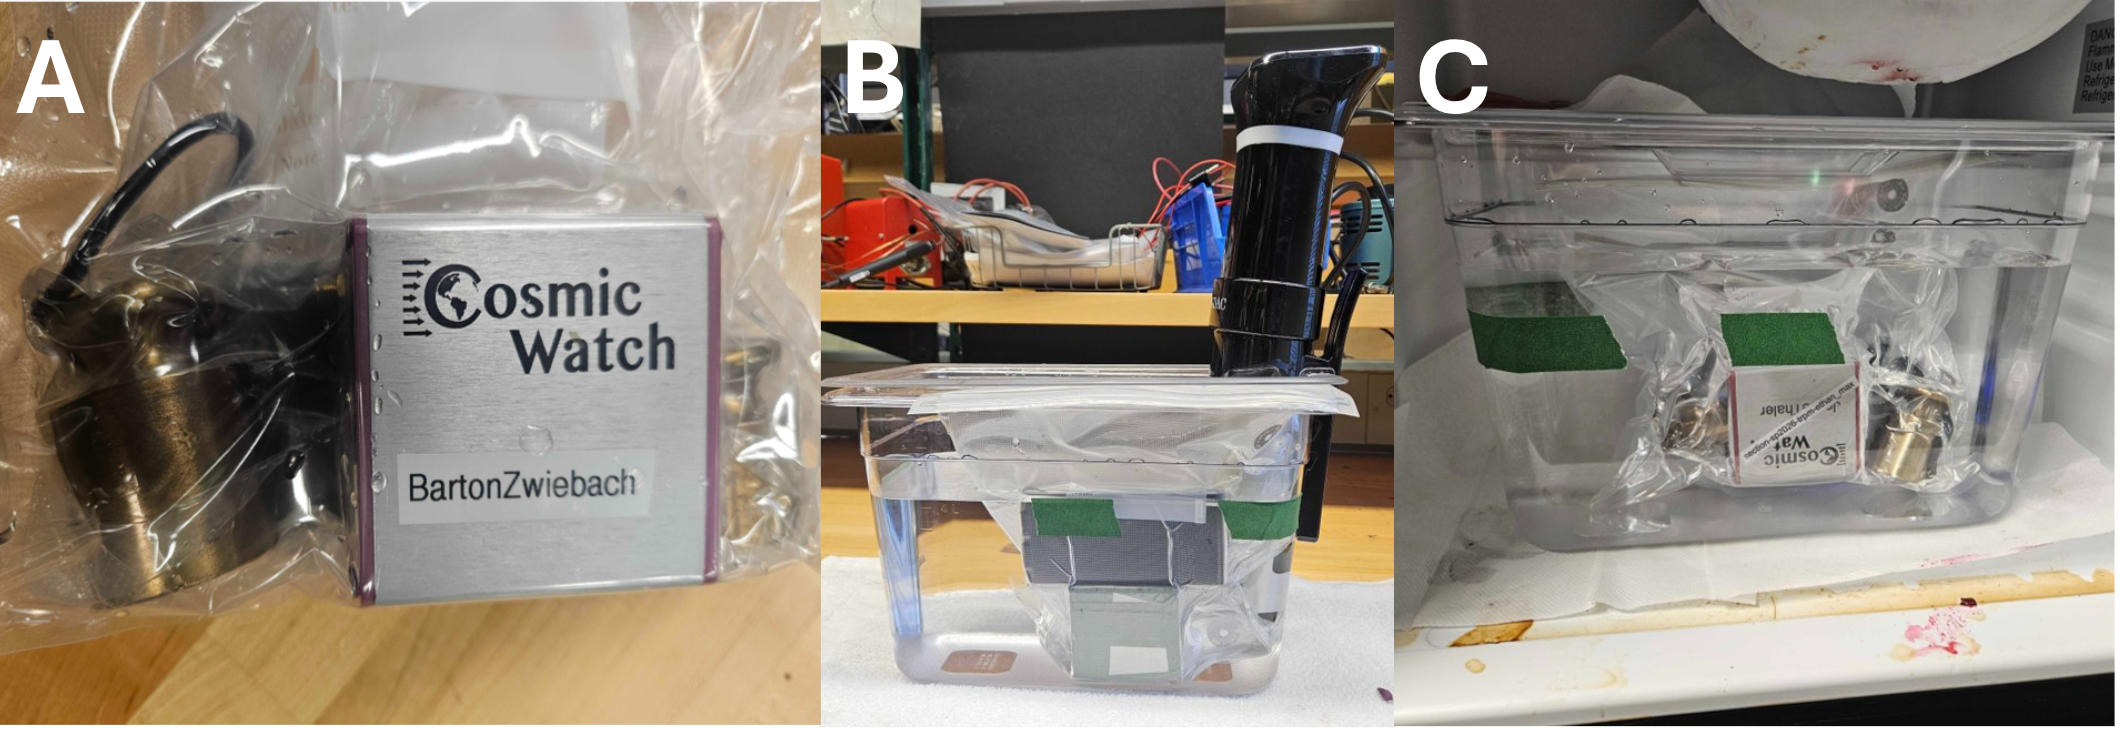
\includegraphics[width=1.0\linewidth]{apparatus.png}
    \caption{The experimental apparatus. (a) The CosmicWatch detector inside its plastic sous-vide bag with brass anchor weights and a USB power bank, prior to immersion. (b) The sous-vide bag is submerged in a plastic water-filled container heated by an immersion-circulator sous-vide cooker, accessing $T = 25$ to $56\,^{\circ}\text{C}$ at $\pm 0.5\,^{\circ}\text{C}$ stability. (c) The same apparatus configuration is placed in a refrigerator and allowed to cool overnight, accessing $T \approx 8.5 \pm 0.5\,^{\circ}\text{C}$.}
    \label{fig:apparatus}
\end{figure*}
\section{Experimental Apparatus and Procedure}


The CW device is used to quantify the total count rate across a range of controlled-temperature conditions. Current pulses produced by the SiPM are amplified by an on-board operational amplifier and digitized by an ATmega328P microcontroller~\cite{cosmicwatch_manual}. For each detection event, the device records the elapsed time since power-on, the on-board temperature, pressure, SiPM response amplitude voltage, and the per-event dead time during which the trigger is inhibited. The experimental observable, the net count rate, is the sum of the intrinsic dark current rate and contributions from ionizing radiation in the environment such as gamma rays. Steps are therefore taken to maintain the background radiation environment as consistent as possible throughout the experiment.

To create a high-temperature environment for the SiPM, the CosmicWatch and an Elecom portable USB power bank are sealed in an airtight plastic \emph{sous-vide} bag, anchored by $500\,\text{g}$ and $100\,\text{g}$ brass weights, and submerged in a water-filled container [Fig.~\ref{fig:apparatus}(a)]. Above-ambient temperatures ($T = 25$ to $56\,^{\circ}\text{C}$) are reached with an Anova immersion sous-vide cooker [Fig.~\ref{fig:apparatus}(b)] stable to $\pm 0.5\,^{\circ}\text{C}$; the low-$T$ point ($T \approx 8.5 \pm 0.5\,^{\circ}\text{C}$) is reached by placing the same container in a refrigerator [Fig.~\ref{fig:apparatus}(c)] for approximately 20 hours. The two configurations are placed in close proximity to minimize differences in the background radiation environment. The power bank is rated to $\sim 60\,^{\circ}\text{C}$, which sets the upper bound of the accessible temperature range.

After cooling in the refrigerator, the CW was powered on and acquired data inside the fridge for approximately 20 minutes. The sous-vide container was then removed from the fridge, and the water temperature was immediately measured using the built-in immersion-cooker thermometer, yielding $T \approx 8.5 \pm 0.5\,^{\circ}\text{C}$. Throughout the experiment, the immersion-cooker water temperature is treated as the ``nominal'' temperature of the CW. The immersion heater was set to $25\,^{\circ}\text{C}$ and the container allowed to equilibrate for approximately 15 minutes. The target temperature was then increased in $5\,^{\circ}\text{C}$ increments up to $55\,^{\circ}\text{C}$, with a 9-minute equilibration window at each setpoint. Over the course of the experiment, the CW detector was observed to power off after 15--20 minutes of submersion, necessitating apparatus rearrangement to turn on the device. Each intervention re-orients the non-isotropic SiPM--scintillator assembly with respect to the background radiation flux, potentially introducing a orientation-dependent systematic effect on the count rate. Five such trials were performed, spanning $8$ to $55\,^{\circ}\text{C}$, each with a different apparatus orientation. Between Trial 4 and Trial 5, the apparatus required minimal adjustment, suggesting reduced systematic divergence between these two trials.

\section{Data and Error Analysis}

The detection data are binned both by the sous-vide nominal temperature during each 9-minute equilibration window and in $1\,^{\circ}\text{C}$ increments according to the internal CW temperature sensor. For each temperature bin, the live observation time accounts for the per-event dead time,
\begin{equation}
    T_{\mathrm{live}} = T_{\mathrm{elapsed}} - \sum_{i=1}^{N} \delta t_{i}^{\,\mathrm{dead}},
    \label{eq:tlive}
\end{equation}
and the dead-time-corrected rate and its statistical uncertainty are
\begin{align}
    R          &= \frac{N}{T_{\mathrm{live}}},           \label{eq:rate}   \\[2pt]
    \sigma_{R} &= \frac{\sqrt{N}}{T_{\mathrm{live}}},    \label{eq:rate_err}
\end{align}
with Eq.~\eqref{eq:rate_err} following from $\sigma_{N} = \sqrt{N}$ for an independent (Poisson) counting process.
\begin{figure}[t]
    \centering
    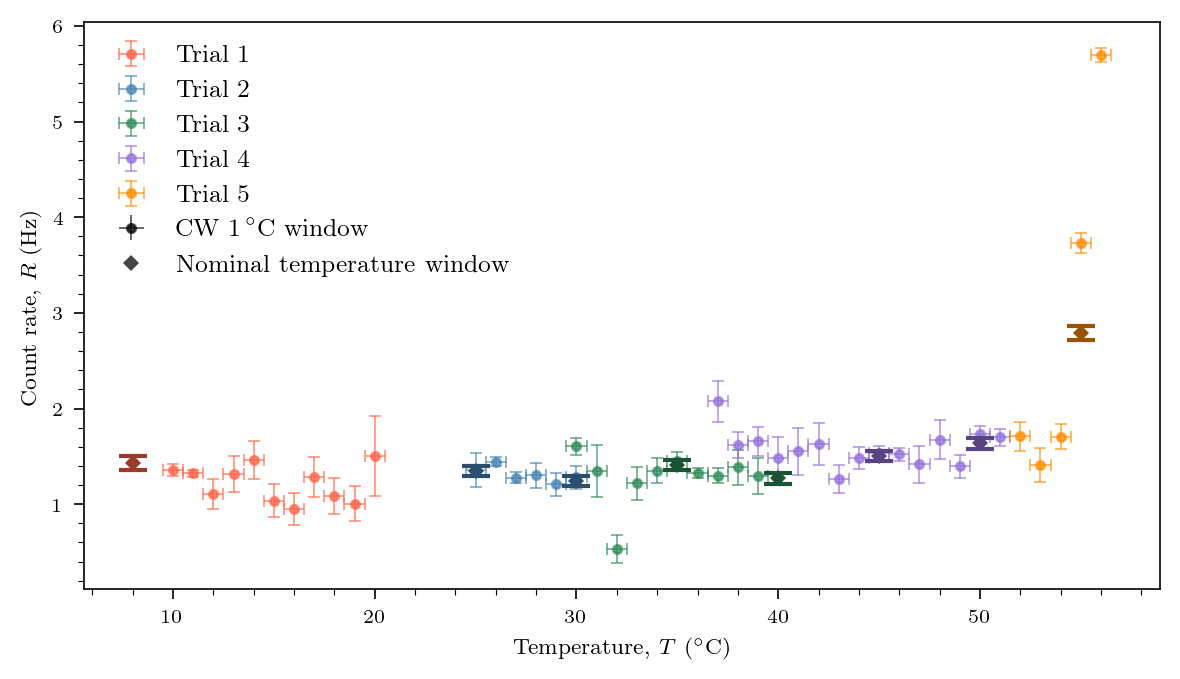
\includegraphics[width=1.0\linewidth]{count_rate_vs_temperature.png}
    \caption{The total count rate $R$ versus temperature $T$, colored by trial. Filled circles denote rates over the nominal $9$\,minute equilibration windows and diamonds denote $1\,^{\circ}\text{C}$-binned rates according to the internal CW temperature sensor. Error bars show the temperature and Poisson statistical uncertainties (Eq.~\ref{eq:rate_err}).}
    \label{fig:rate}
\end{figure}
Figure~\ref{fig:rate} summarizes $R(T)$ across all five trials for both binning methods. Below $50\,^{\circ}\text{C}$ the rate is approximately constant at $R \approx 1.3\,\text{Hz}$. The nominal-temperature rates are consistent with the CW internal temperature rates, supporting the reliability of the on-board temperature sensor. At $T = 55\,^{\circ}\text{C}$ the discrepancy between binning methods becomes larger due to the sharp rise in $R$.
We investigate whether this increase can be explained by apparatus- or environment-dependent systematic effects. An estimate of the orientation-induced apparatus variation between trials is obtained by comparing the count rates of different trials at the same temperature bin, yielding an average variation of $\Delta R_{\mathrm{app}} = 0.4 \pm 0.2\,\text{Hz}$. This is small compared to the overall rise at high temperature. The CW internal pressure measurement is examined in Fig.~\ref{fig:pressure} for similar trends.
\begin{figure}[t]
    \centering
    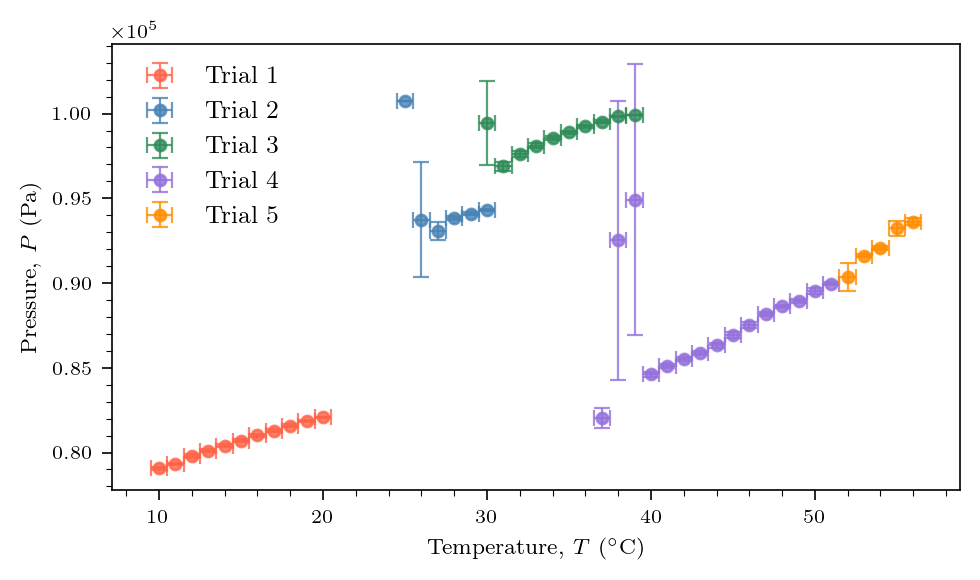
\includegraphics[width=1.0\linewidth]{pressure_vs_temperature.png}
    \caption{On-board pressure $P$ versus temperature $T$ across the five trials. Discontinuities between trials reflect re-sealing of the bag. No anomalous feature is observed at $T \geq 50\,^{\circ}\text{C}$, ruling out a pressure-induced cause for the rate spike in Fig.~\ref{fig:rate}.}
    \label{fig:pressure}
\end{figure}
Ideal-gas behavior is evident in the linear dependence of pressure on temperature, and the pressure is significantly affected by each apparatus rearrangement. However, at the transition from Trial 4 to Trial 5, where minimal adjustment occurred, the pressure increases continuously with temperature. These observations indicate that the rise in count rate at high temperature cannot be explained by apparatus-induced effects.

Comparing the count rate inside the fridge ($T = 8.5\,^{\circ}\text{C}$) with that immediately outside ($8.5\,^{\circ}\text{C} < T < 25\,^{\circ}\text{C}$), the difference is also small, indicating that systematic shifts associated with the different background environments can be neglected.

The temperature--rate data are then fit to the SRH model of Eq.~\ref{eq:srh} on a logarithmic Arrhenius plot, shown in Fig.~\ref{fig:arrhenius}.
\begin{figure}[t]
    \centering
    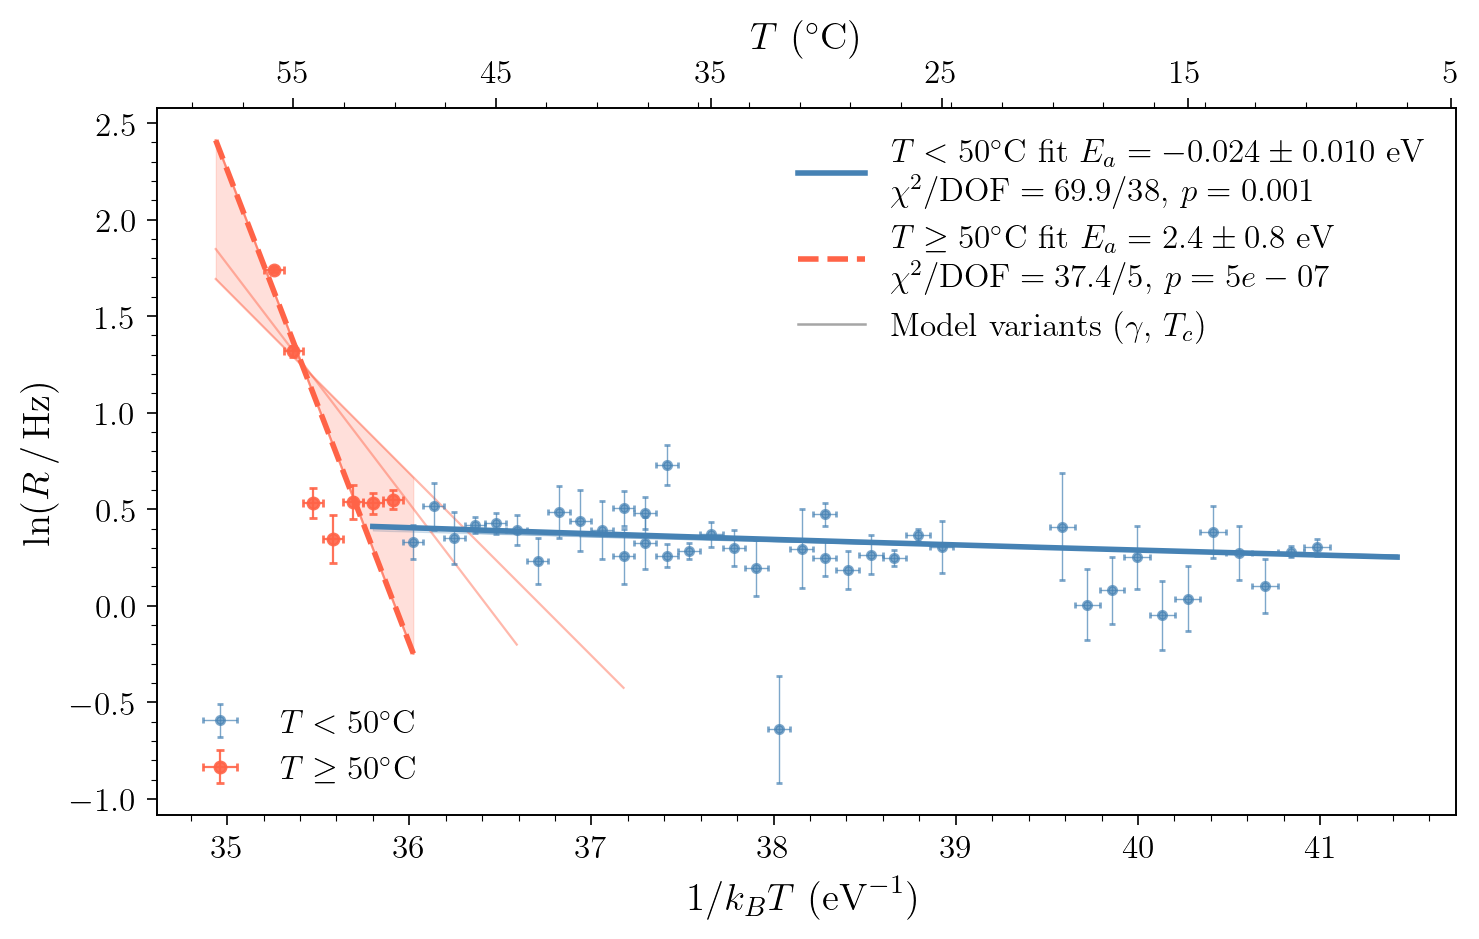
\includegraphics[width=1.0\linewidth]{arrhenius_systematics.png}
    \caption{Arrhenius plot of $\ln R$ versus $1/k_B T$. Blue points ($T < 50\,^{\circ}\text{C}$) and red points ($T \geq 50\,^{\circ}\text{C}$) are fit independently to the linearized SRH form derived from Eq.~\ref{eq:srh} via ODR. The shaded envelope and light solid lines show the spread of fits over the systematic variants $\gamma \in \{1,2,3\}$ and $T_c \in \{40, 45, 50\}\,^{\circ}\text{C}$.}
    \label{fig:arrhenius}
\end{figure}
The qualitatively different behavior below and above $T_c = 50\,^{\circ}\text{C}$ motivates an independent two-regime fit of the linearized SRH form using SciPy's orthogonal-distance-regression (ODR). The low-$T$ fit yields $E_a^{\mathrm{low}} = -0.024 \pm 0.01\,\text{(stat.)}\,\text{eV}$ with $p = 1.2\times 10^{-3}$, while the high-$T$ fit yields $E_a^{\mathrm{high}} = 2.4 \pm 0.8\,\text{(stat.)\,eV}$ with $p = 5\times 10^{-7}$ (the corresponding $\chi^2$ and DOF appear in the legend of Fig.~\ref{fig:arrhenius}). Both $p$-values fall well below conventional acceptance thresholds, indicating that systematic variance between apparatus configurations and the limited number of high-$T$ data points are not fully captured by the per-bin Poisson uncertainty.

The uncertainty in $E_a$ due to the model parameters, namely the regime cutoff $T_c$ and the power-law index $\gamma$, is quantified by repeating the fit while varying these parameters. With $\gamma \in \{1, 2, 3\}$, half the spread,
\begin{equation}
    \sigma_{\mathrm{sys}}^{(\gamma)} = \frac{|E_a(\gamma=3) - E_a(\gamma=1)|}{2},
    \label{eq:sys_gamma}
\end{equation}
gives $\sigma_{\mathrm{sys}}^{(\gamma)} = 0.03\,\text{eV}$ in both regimes. Similarly, repeating the fit with $T_c \in \{40, 45, 50\}\,^{\circ}\text{C}$ and taking half the full range,
\begin{equation}
    \sigma_{\mathrm{sys}}^{(T_c)} = \frac{\displaystyle\max_{i}\,E_a(T_c^{(i)}) - \min_{i}\,E_a(T_c^{(i)})}{2},
    \label{eq:sys_cutoff}
\end{equation}
yields $0.008\,\text{eV}$ (low-$T$) and $0.8\,\text{eV}$ (high-$T$). The two regime fits are visually rendered in Fig.~\ref{fig:arrhenius} as the colored envelopes around the nominal fit lines, illustrating the sensitivity of the high-$T$ activation energy to the assumed model. The two systematic contributions are combined in quadrature, giving $\sigma_{\mathrm{sys}} = 0.03\,\text{eV}$ (low-$T$) and $0.8\,\text{eV}$ (high-$T$).


\section{Results and Discussion}
The systematic uncertainties accounted for in this study are summarized in Table~\ref{tab:systematics}.

\begin{table}[h]
\centering
\caption{Sources of statistical and systematic uncertainty on $E_a$ for the two temperature regimes. Values are quoted in eV; sources are listed by decreasing magnitude.}
\label{tab:systematics}
\begin{tabular}{lcc}
\hline\hline
Source
  & Low-$T$ ($T < 50\,^{\circ}\text{C}$)
  & High-$T$ ($T \geq 50\,^{\circ}\text{C}$) \\
\hline
$T_c$ (regime cutoff)
  & $\pm 0.008$
  & $\pm 0.8$ \\
$\gamma$ (power-law index)
  & $\pm 0.03$
  & $\pm 0.03$ \\
\hline
$\sigma_{\mathrm{sys}}$ 
  & $\pm 0.03$
  & $\pm 0.8$ \\
$\sigma_{\mathrm{stat}}$ (ODR)
  & $\pm 0.01$
  & $\pm 0.8$ \\
\hline
$\sigma_{\mathrm{total}}$ 
  & $\pm 0.03$
  & $\pm 1$ \\
\hline\hline
\end{tabular}
\end{table}

Combining statistical and systematic contributions in quadrature, we report the activation energies from the SRH model as
\begin{align}
    E_a^{\mathrm{low}}  &= -0.024 \pm 0.01\,\text{(stat.)} \pm 0.03\,\text{(sys.)}\,\mathrm{eV}, \label{eq:Ea_low}\\[2pt]
    E_a^{\mathrm{high}} &= 2.4 \pm 0.8\,\text{(stat.)} \pm 0.8\,\text{(sys.)}\,\mathrm{eV}. \label{eq:Ea_high}
\end{align}

The high-$T$ result agrees with the Pagano \emph{et al.} value $E_a = 1.18\,\text{eV}$~\cite{pagano2012} at $1.2\sigma$, while the low-$T$ result disagrees with their corresponding low-temperature value $E_a = 0.57\,\text{eV}$ by approximately $20\sigma$. Despite the low fit probabilities, the high-$T$ agreement suggests a regime in which the activation energy of pair generation is set by the silicon band gap, as theoretically predicted. Several explanations are plausible for the low-$T$ discrepancy. First, the dark current rate cannot be separated from the total count rate in this experiment; the flat count rate from $T = 8$ to $50\,^{\circ}\text{C}$ may therefore reflect ambient background radiation dominating over the dark current rate in this regime. Second, the CW has a software-defined minimum trigger voltage of $5$\,mV; SiPM events producing avalanche pulses below this threshold are not recorded. The vast majority of SiPM dark current pulses likely fall below this cutoff, given that the room-temperature dark count rate for the CW SiPM is reported to be $\sim 30\,\text{kHz/mm}^2$~\cite{cosmicwatch_manual}, several orders of magnitude larger than the observed rates. Third, the SiPM material itself differs from that of Pagano \emph{et al.}; their STMicroelectronics device may have a higher impurity-defect concentration than the OnSemi CW SiPM, producing more SRH-mediated dark current at low temperature. Lowering the CW trigger threshold and characterizing the energy profile of dark current, together with improved background shielding, would help disentangle these effects.

To further reduce systematic error from apparatus variation, the cause of the CW or battery pack powering off under submersion warrants investigation, as resolving this would eliminate the need to conduct multiple trials. Longer thermal-equilibration windows would also allow more data to be acquired at each setpoint, reducing the per-bin Poisson uncertainty.

%%%%%%%%%%%%%%%%%%%%%%%%%%%%%%%%%%%%%%%%%%%%%%%%%%%%%%%%%%%%%%%%%%%%%%%%%%%%%
\section{Conclusions}

The activation energies for SRH pair generation obtained in this study are given in Eqs.~\eqref{eq:Ea_low} and \eqref{eq:Ea_high}, and the systematic uncertainties are summarized in Table~\ref{tab:systematics}. In the high-$T$ ($T \geq 50\,^{\circ}\text{C}$) regime we observe a sharp rise in the count rate that cannot be explained by apparatus-dependent effects, and the extracted activation energy is consistent with pair generation mediated by the silicon band gap, in agreement with Pagano \emph{et al.} A definitive physical explanation for the low-$T$ behavior, however, requires further investigation. Overall, we confirm the robustness of the CosmicWatch desktop muon detector against temperature-dependent dark current for $T = 8$ to $50\,^{\circ}\text{C}$..


%%%%%%%%%%%%%%%%%%%%%%%%%%%%%%%%%%%%%%%%%%%%%%%%%%%%%%%%%%%%%%%%%%%%%%%%%%%%%
\begin{acknowledgments}
The authors thank Max Misterka for collaboration during the data-collection phase of this experiment, and the Junior Lab staff, comprising Prof.\ Janet Conrad, Jixiang Yang, Simon Rothman, Vinh Tran, Atissa Banuazizi, Dr.\ Sean Robinson, Dr.\ Aaron Pilarcik, and Cory Romanov, for providing the experimental equipment and laboratory manual and for their guidance and technical support throughout. The AI tools ChatGPT and Claude Code were used to assist with literature review and to generate the analysis code and figures, as well as assist with the writing style and formatting of this paper. The source code accompanying this paper can be found at~\cite{suresh_sipm_jlab}.
\end{acknowledgments}

%%%%%%%%%%%%%%%%%%%%%%%%%%%%%%%%%%%%%%%%%%%%%%%%%%%%%%%%%%%%%%%%%%%%%%%%%%%%%
\bibliography{sipm}


%%%%%%%%%%%%%%%%%%%%%%%%%%%%%%%%%%%%%%%%%%%%%%%%%%%%%%%%%%%%%%%%%%%%%%%%%%%%%
\clearpage
\end{document}

